\documentclass[a4paper, final]{article}

% ============================================================
% НАСТРОЙКИ (settings.tex)
% ============================================================
\usepackage{fontspec}
\setmainfont{Times New Roman}
\setmonofont{Courier New}
\usepackage[14pt]{extsizes}

\usepackage{polyglossia}
\setdefaultlanguage{russian}

\usepackage[left=20mm, top=20mm, right=20mm, bottom=20mm, footskip=10mm]{geometry}
\usepackage{ragged2e}
\usepackage{indentfirst}
\usepackage{hyperref}
\usepackage{graphicx}
\usepackage{tikz}
\usepackage{caption}
\usepackage{subcaption}
\usepackage{xcolor}
\usepackage{listings}
\usepackage{algorithm}
\usepackage{algorithmic}
\usepackage{soul}

\definecolor{codegray}{gray}{0.95}
\definecolor{codered}{rgb}{0.6,0,0}
\definecolor{codeblue}{rgb}{0,0,0.6}
\definecolor{codegreen}{rgb}{0,0.5,0}

\lstdefinestyle{common}{
  basicstyle=\ttfamily\small,
  backgroundcolor=\color{codegray},
  frame=single,
  numbers=left,
  numberstyle=\tiny\color{gray},
  stepnumber=1,
  numbersep=6pt,
  showspaces=false,
  showstringspaces=false,
  showtabs=false,
  tabsize=2,
  breaklines=true,
  breakatwhitespace=true,
  captionpos=b,
  keywordstyle=\color{codeblue}\bfseries,
  commentstyle=\color{codegreen}\itshape,
  stringstyle=\color{codered}
}

\lstdefinestyle{bashstyle}{
  style=common,
  language=bash
}

\lstdefinestyle{cstyle}{
    style=common,
    language=C++,
    inputencoding=utf8,
    extendedchars=true,
    keepspaces=true,
    columns=fullflexible,
	    literate={а}{{\selectfont\char224}}1
             {б}{{\selectfont\char225}}1
             {в}{{\selectfont\char226}}1
             {г}{{\selectfont\char227}}1
             {д}{{\selectfont\char228}}1
             {е}{{\selectfont\char229}}1
             {ё}{{\"e}}1
             {ж}{{\selectfont\char230}}1
             {з}{{\selectfont\char231}}1
             {и}{{\selectfont\char232}}1
             {й}{{\selectfont\char233}}1
             {к}{{\selectfont\char234}}1
             {л}{{\selectfont\char235}}1
             {м}{{\selectfont\char236}}1
             {н}{{\selectfont\char237}}1
             {о}{{\selectfont\char238}}1
             {п}{{\selectfont\char239}}1
             {р}{{\selectfont\char240}}1
             {с}{{\selectfont\char241}}1
             {т}{{\selectfont\char242}}1
             {у}{{\selectfont\char243}}1
             {ф}{{\selectfont\char244}}1
             {х}{{\selectfont\char245}}1
             {ц}{{\selectfont\char246}}1
             {ч}{{\selectfont\char247}}1
             {ш}{{\selectfont\char248}}1
             {щ}{{\selectfont\char249}}1
             {ъ}{{\selectfont\char250}}1
             {ы}{{\selectfont\char251}}1
             {ь}{{\selectfont\char252}}1
             {э}{{\selectfont\char253}}1
             {ю}{{\selectfont\char254}}1
             {я}{{\selectfont\char255}}1
             {А}{{\selectfont\char192}}1
             {Б}{{\selectfont\char193}}1
             {В}{{\selectfont\char194}}1
             {Г}{{\selectfont\char195}}1
             {Д}{{\selectfont\char196}}1
             {Е}{{\selectfont\char197}}1
             {Ё}{{\"E}}1
             {Ж}{{\selectfont\char198}}1
             {З}{{\selectfont\char199}}1
             {И}{{\selectfont\char200}}1
             {Й}{{\selectfont\char201}}1
             {К}{{\selectfont\char202}}1
             {Л}{{\selectfont\char203}}1
             {М}{{\selectfont\char204}}1
             {Н}{{\selectfont\char205}}1
             {О}{{\selectfont\char206}}1
             {П}{{\selectfont\char207}}1
             {Р}{{\selectfont\char208}}1
             {С}{{\selectfont\char209}}1
             {Т}{{\selectfont\char210}}1
             {У}{{\selectfont\char211}}1
             {Ф}{{\selectfont\char212}}1
             {Х}{{\selectfont\char213}}1
             {Ц}{{\selectfont\char214}}1
             {Ч}{{\selectfont\char215}}1
             {Ш}{{\selectfont\char216}}1
             {Щ}{{\selectfont\char217}}1
             {Ъ}{{\selectfont\char218}}1
             {Ы}{{\selectfont\char219}}1
             {Ь}{{\selectfont\char220}}1
             {Э}{{\selectfont\char221}}1
             {Ю}{{\selectfont\char222}}1
             {Я}{{\selectfont\char223}}1,
}

\linespread{0.98}

\definecolor{link_color}{HTML}{0000EE}

\hypersetup{
    colorlinks=true,
    linkcolor=link_color,
    urlcolor=link_color,
    citecolor=link_color
}

% ============================================================
% ДОКУМЕНТ
% ============================================================
\begin{document}

% ============================================================
% ТИТУЛЬНЫЙ ЛИСТ (title.tex)
% ============================================================
{
\thispagestyle{empty}
\begin{center}
    \hfill \break
    \hfill \break
    МИНИСТЕРСТВО НАУКИ И ВЫСШЕГО ОБРАЗОВАНИЯ РОССИЙСКОЙ ФЕДЕРАЦИИ\\[5 pt]
    Федеральное государственное автономное образовательное учреждение высшего образования
    «Санкт-Петербургский политехнический университет Петра Великого»\\[10 pt]
    Институт компьютерных наук и кибербезопасности\\ [5 pt]
	Высшая школа технологий искусственного интеллекта \\ [5 pt]
    Направление: 02.03.01 Математика и компьютерные науки\\[30pt]

    {\large ОТЧЕТ ПО Лабораторной работе №3}\\[10 pt]
    {\large по дисциплине Программирование микроконтроллеров}\\[40 pt]
    {\large\bf События и прерывания..}
\end{center}

\vspace{110 pt}

\begin{tabular*}{460pt}{@{\extracolsep{\fill}} l r}
     Студент,\tabularnewline группы 5130201/40003 &  \line(1,0){100} \quad Адиатуллин Т.Р\\
     & \\
     Руководитель,\tabularnewline Преподаватель &  \line(1,0){100} \quad Вербова Н. М.\\
     & \\
     & \\
     & \\
     & \guillemotleft \line(1,0){30} \guillemotright \line(1,0){100} \, 2026 \,г.

\end{tabular*} \\

\vfill

\begin{center}
    Санкт-Петербург, 2026
\end{center}
\newpage
}

\tableofcontents
\newpage

% ============================================================
% ОСНОВНОЕ СОДЕРЖАНИЕ (base.tex)
% ============================================================
\section{Цель работы}
Ознакомление с основными приемами работы с документацией при
составлении программ для микроконтроллеров. Приобретение навыков работы с
осциллографом и оценочной платой MCBSTM32F200 в качестве измерительного
генератора	.

\section{Постановка задачи}
Используя библиотеки Keil µVision5, разработать
программу для микроконтроллера (МК) STM32F200, которая включает и выключает
светодиод.

\section{Алгоритм работы программы}

Данный раздел описывает последовательность действий, необходимых для разработки и реализации проекта на базе микроконтроллера STM32F207IGHx в среде Keil~µVision5. Алгоритм включает этапы инициализации проекта, настройки портов ввода–вывода, реализации мигания светодиода и модификации программы для создания эффекта «бегущего огня».

\subsection{Инициализация проекта}
\begin{itemize}
    \item Создание нового проекта в среде Keil \(\mu\)Vision5.
    \item Выбор микроконтроллера \textbf{STM32F207IGHx}.
    \item Настройка параметров проекта, включая поддержку ядра (\textit{CMSIS CORE}), запуск (\textit{Startup}) и настройки HAL.
    \item Подключение библиотеки \texttt{stm32f2xx.h}, где хранится информация обо всех адресах регистров.
\end{itemize}

\subsection{Настройка порта GPIOG}
\begin{itemize}
    \item Включение тактирования порта GPIOG через регистр \texttt{RCC\_AHB1ENR}.
    \item Переключение режима работы GPIOG в режим вывода через регистр \texttt{GPIOG\_MODER}.
\end{itemize}

\subsection{Используемые переменные и регистры}
\begin{description}
    \item \texttt{RCC->AHB1ENR} — включает тактирование периферийных устройств, используется для активации GPIOG.
    \item \texttt{GPIOG->MODER} — задает режим работы пина PG7 (настроен как выход).
    \item \texttt{GPIOG->ODR} — управляет включением и выключением светодиода.
\end{description}

\subsection{Реализация мигания светодиода}
\begin{enumerate}
    \item Установка бита PG7 в \texttt{GPIOG\_ODR} в "1" (включение светодиода).
    \item Ожидание задержки для визуального восприятия мигания.
    \item Сброс бита PG7 в \texttt{GPIOG\_ODR} в "0" (выключение светодиода).
    \item Повторение цикла для непрерывного мигания.
\end{enumerate}

\section{Ответ на вопросы до работы с осциллографом}
\begin{enumerate}
	\item A: 8x10 делений
	\item B: 5V
	\item C: Масштаб станет равным 5В/деление, а сигнал будет занимать 2 вертикальных деления
	\item A: 500 µS
	\item B: 1250 Hz
\end{enumerate}

\section{Полученные результаты}
\begin{itemize}
	\item Успешно создан проект в Keil μVision5.
	\item Разработана программа, которая управляет светодиодом на оценочной плате MCBSTM32F200.
	\item Программа корректно работает: светодиод мигает с заданной частотой.
	\item Модифицированная программа с бегущей строкой также успешно протестирована.
\end{itemize}

\newpage

\section*{Код программы}

\begin{lstlisting}[style=cstyle, caption={Основная функция программы}]
#include "stm32f2xx.h" // Подключаем библиотеку, где лежат адреса всех регистров

// Функция реализации задержки
void delay ()
{
    unsigned long i; // Переменная для счетчика цикла
		// Цикл, который просто выполняется много раз, чтобы создать задержку
    for(i=0; i<2000000; i++){} 
}

// Главная функция программы
int main ()
{
    RCC->AHB1ENR |= 1ul<<6; 
    GPIOG->MODER = (GPIOG->MODER & ~1ul<<15) | 1ul<<14;

    for (;;)
    {
        GPIOG->ODR |= 1ul<<7;
        delay ();
        GPIOG->ODR &= ~1ul<<7;
        delay ();
    }
}
\end{lstlisting}

\section{Работа с осциллографом}
Для измерения был получен снимок нескольких тактов сигнала:
\begin{itemize}
	\item Размах сигнала: 3.2 В
	\item Период сигнала: 1.5 с
	\item Частота сигнала: 0.66 Гц
	\item Ширина положительного уровня: 0.75 с
	\item Ширина отрицательного уровня: 0.75 с
	\item Коэффициент заполнения: 0.5
\end{itemize}
\newpage

\begin{figure}[h!]
\centering
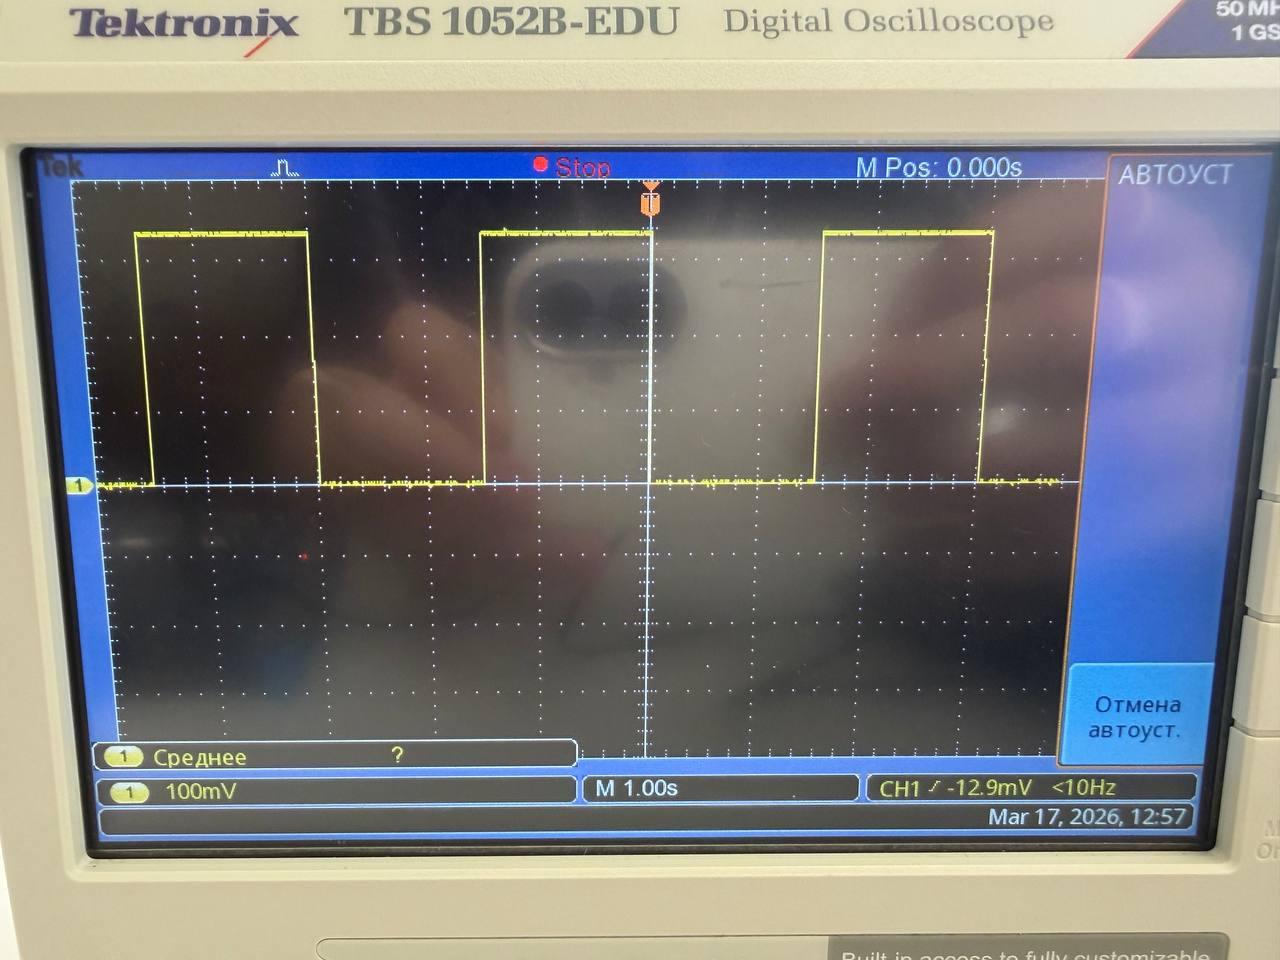
\includegraphics[width=0.9\textwidth]{Photo/1.jpg}
\end{figure}
Для измерения времени нарастания формы волны был получен другой
снимок.
Время нарастания от 20\% сигнала до 80\%: 6.5 нс

\begin{figure}[h!]
\centering

\includegraphics[width=0.9\textwidth]{Photo/2.jpg}
\end{figure}
Для измерения времени затухания формы волны был получен другой снимок.
Время затухания от 20\% сигнала до 80\%: 6.5 нс

\begin{figure}[h!]
\centering

\includegraphics[width=0.9\textwidth]{Photo/3.jpg}
\end{figure}

Далее нужно было изменить задержки в программе так, чтобы значение
скважности стало 1/3. Для этого нужно было задержку после включения
светодиода увеличить в 2 раза.

\begin{figure}[h!]
\centering
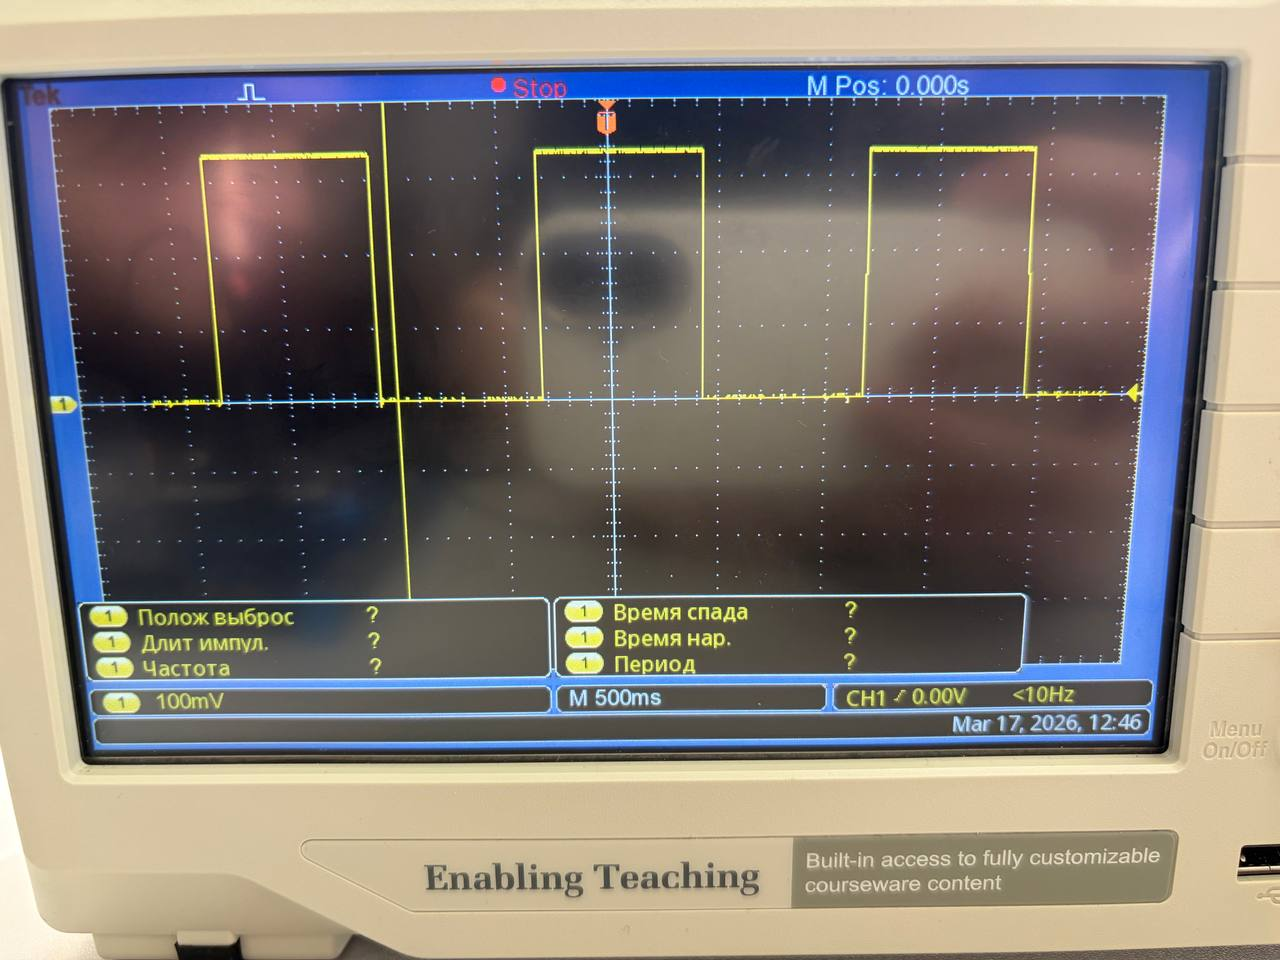
\includegraphics[width=0.9\textwidth]{Photo/4.jpg}
\end{figure}

\newpage

\section{Результаты работы с осциллографом}

\textbf{1. Изученные концепции}
Применение библиотечных функций для управления периферийными модулями микроконтроллера STM32F200. Методики проведения измерений электрических сигналов с использованием осциллографического оборудования. Теоретические и практические аспекты реализации широтно-импульсной модуляции (ШИМ) для управления исполнительными устройствами.

\textbf{2. Параметры осциллографа}
\begin{enumerate}
    \item 10 В
    \item 500 мкс
    \item 40 В
    \item 1000 мкс
    \item 1000 Гц
\end{enumerate}

\vspace{1em}

\textbf{3. Проведенные эксперименты}
\begin{enumerate}
    \item \textbf{ШИМ модулятор.} \\
    \textit{Параметр:} амплитуда и частота напряжения.

    \item \textbf{Анализ работы генератора прямоугольных импульсов.} \\
    \textit{Параметр:} скважность и частота сигнала.

    \item \textbf{Изучение работы таймера микроконтроллера.} \\
    \textit{Параметр:} время включения и выключения сигнала.

    \item \textbf{Модуляция светодиода.} \\
    \textit{Параметр:} коэффициент заполнения ШИМ.

    \item \textbf{Проектирование схемы генератора импульсов.} \\
    \textit{Параметр:} время нарастания и спада сигнала.
\end{enumerate}

\vspace{1em}

\textbf{4. Итоговое значение}
\begin{itemize}
    \item 3.33 Гц
\end{itemize}

\newpage

% ============================================================
% ЗАКЛЮЧЕНИЕ (result.tex)
% ============================================================
\addcontentsline{toc}{section}{Заключение}
\section*{Заключение}

В ходе работы был создан проект в среде Keil µVision, разработана программа на языке C и выполнен анализ сигнала с использованием осциллографа. Реализована последовательная смена состояний светодиода G7 на микроконтроллере STM32F200. Получены характеристики сигнала: частота, амплитуда, период, время нарастания и спада. Установлено, что время нарастания сигнала примерно равно времени его спада.

\newpage

\end{document}